\section{Comparison and interpretation of results for the train}

The purpose of this section is to interpret and compare results on different pictures deblurred by the three methods of deconvolution : Lucy-Richardson, Wiener and regularization. We will test essentially ideal images artificially blurred in order to isolate the influence of certain parameters. Although most of the images used are not taken inside a train as it indicated, the assumption of a linear motion blur is well respected and we are therefore in the first case treated (the train).

\subsection{Noise influence}

We are interested in deblurring a original image with noise (that is independent of signal). Three different cases are considered: the original image without noise, with Gaussian noise (mean equals $0$ and variance $0.01$) and with (very light) speckle noise\footnote{noise added by $J = I + n*I$, where $n$ is uniformly distributed random noise with mean 0 and variance 0.04\cite{mathWorksNoise}}. The original image has been artificially blurred and pictures are resized during treatment (see section ref{sec:RealTime}). The noise is inserted by predefined functions of Matlab. The results are shown in figure \ref{fig:AllNoises}. 

\begin{figure}[h!]
\centering
\begin{subfigure}{0.32\textwidth}
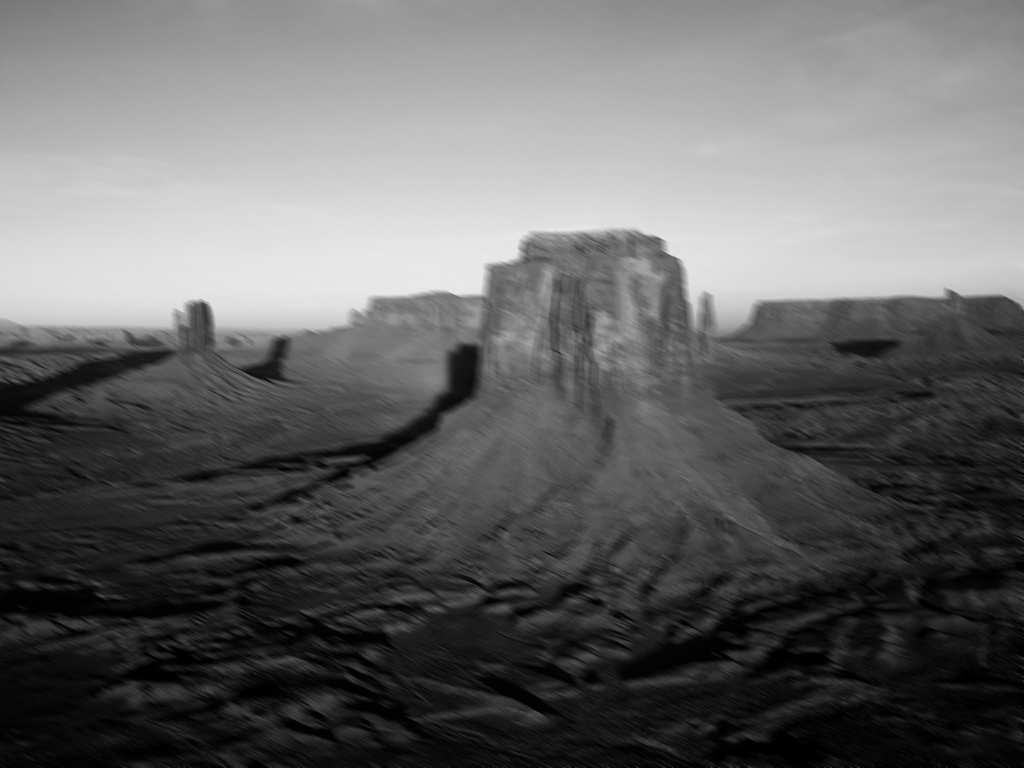
\includegraphics[width= \textwidth]{../Images/Results/desert/Normal/input.png}
\caption{Original image whithout noise}
\label{fig:NormalI}
\end{subfigure}
~
\begin{subfigure}{0.32\textwidth}
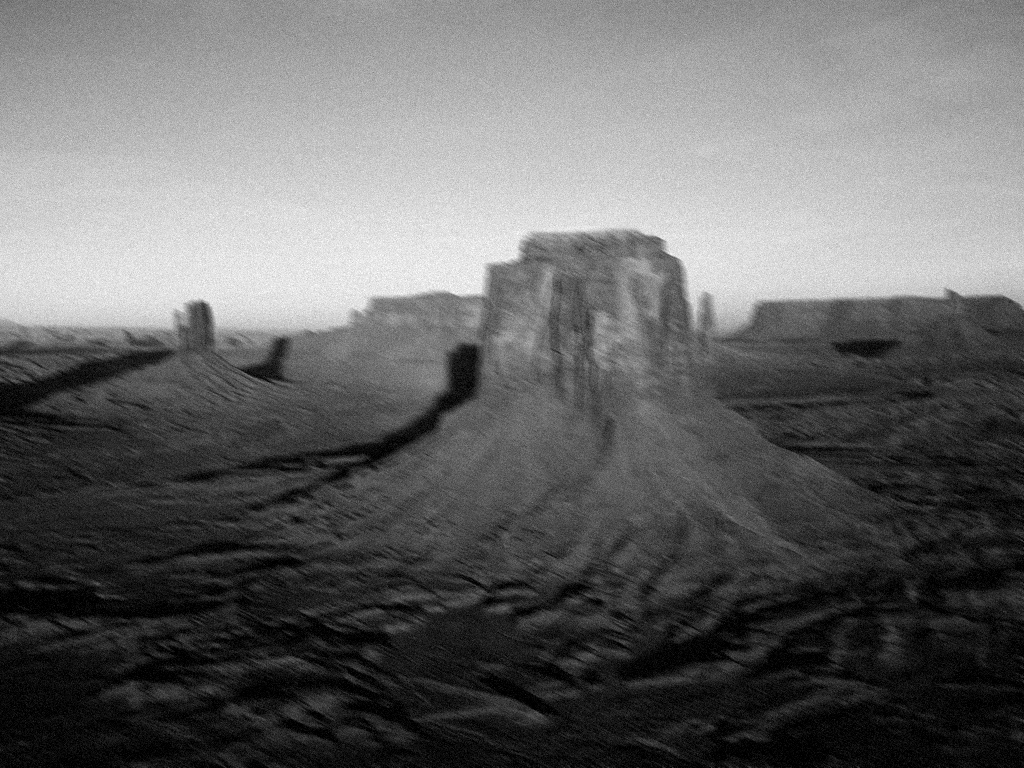
\includegraphics[{width= \textwidth}]{../Images/Results/desert/Gauss/input.png}
\caption{Original image whith Gaussian noise ($\mu = 0$, $\sigma = 0.01$)}
\label{fig:GaussI}
\end{subfigure}
~
\begin{subfigure}{0.32\textwidth}
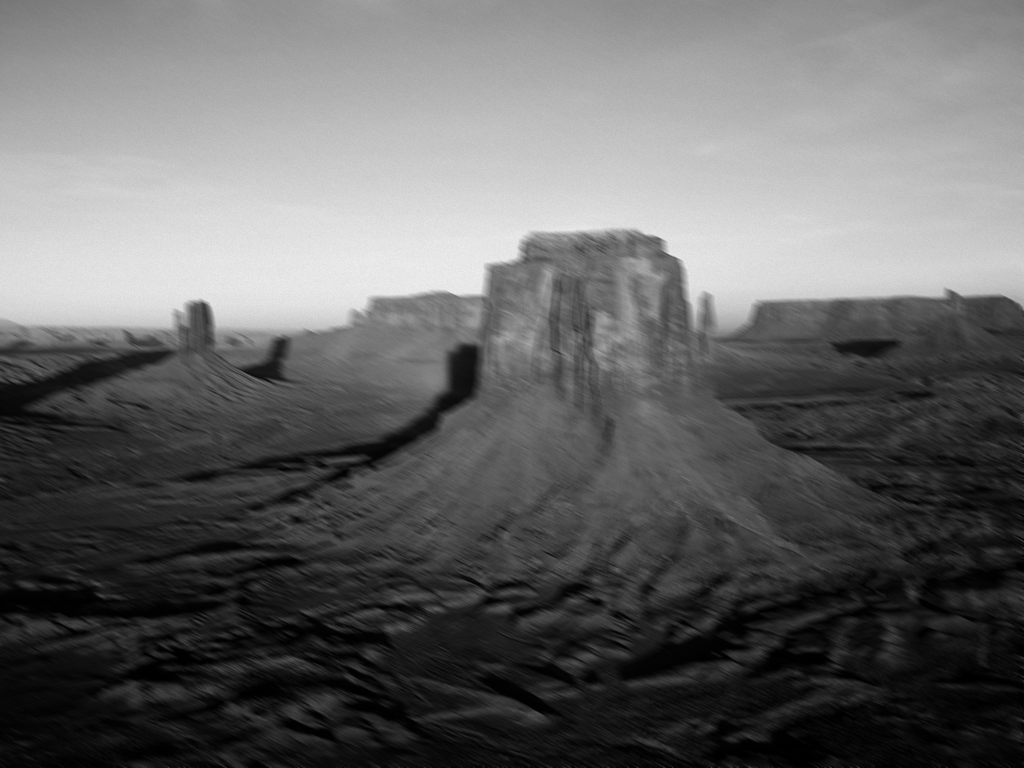
\includegraphics[{width= \textwidth}]{../Images/Results/desert/Speckle/input.png}
\caption{Original image whith Speckle noise}
\label{fig:SpeckleI}
\end{subfigure}
~
\begin{subfigure}{0.32\textwidth}
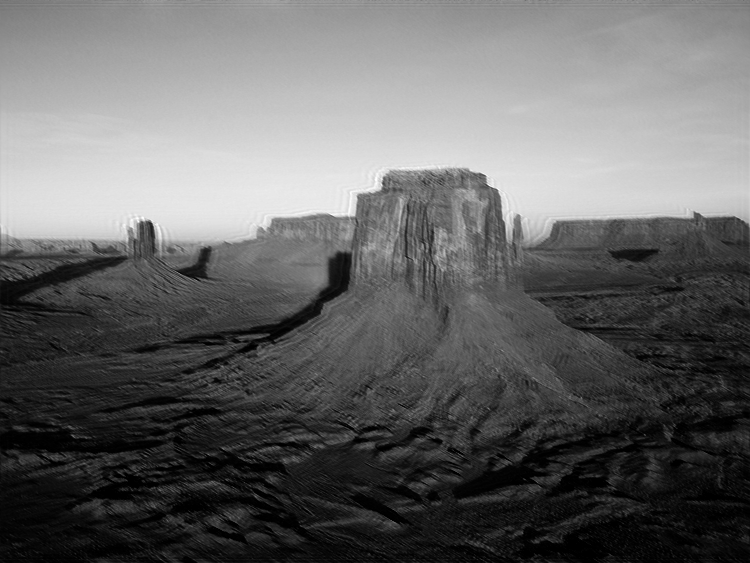
\includegraphics[{width= \textwidth}]{../Images/Results/desert/Normal/L.png}
\caption{Image deblurred with Lucy (no noise)}
\label{fig:NormalL}
\end{subfigure}
~
\begin{subfigure}{0.32\textwidth}
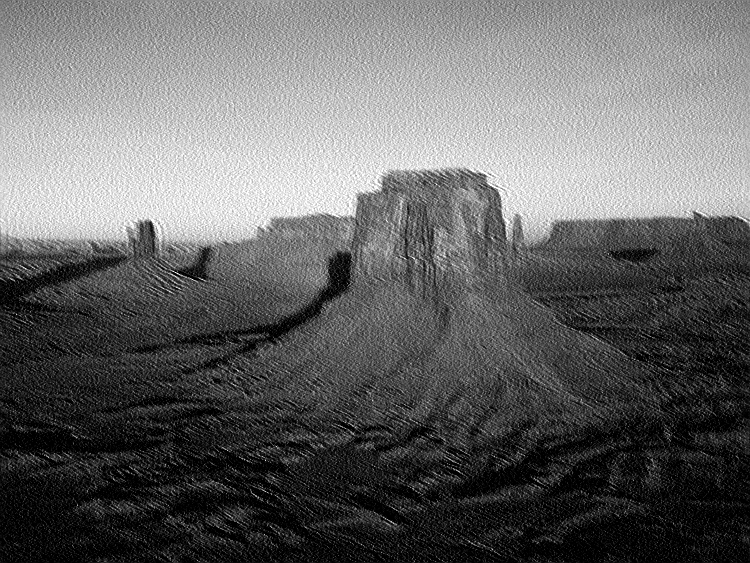
\includegraphics[{width= \textwidth}]{../Images/Results/desert/Gauss/L.png}
\caption{Image deblurred with Lucy (Gaussian noise)}
\label{fig:GaussL}
\end{subfigure}
~
\begin{subfigure}{0.32\textwidth}
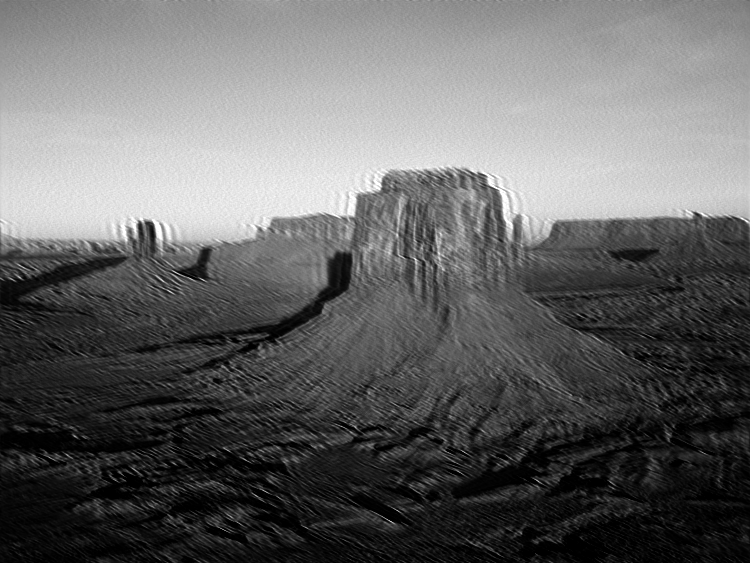
\includegraphics[{width= \textwidth}]{../Images/Results/desert/Speckle/L.png}
\caption{Image deblurred with Lucy (Speckle noise)}
\label{fig:SpeckleL}
\end{subfigure}
~
\begin{subfigure}{0.32\textwidth}
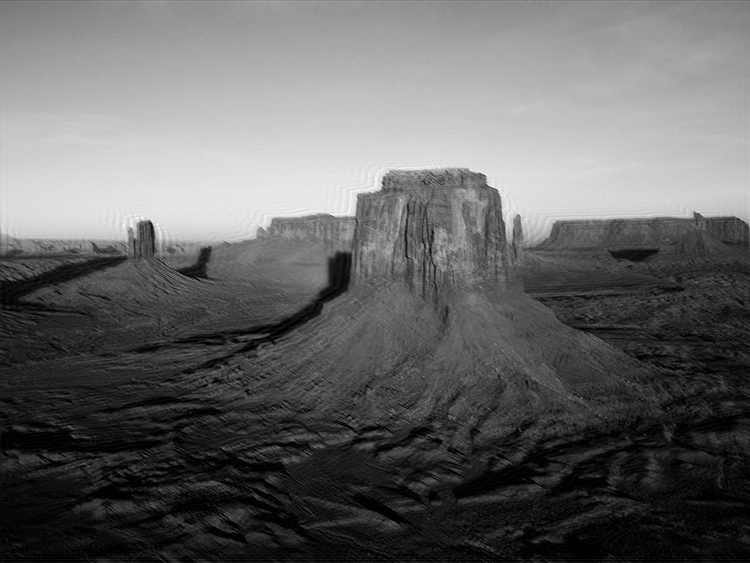
\includegraphics[{width= \textwidth}]{../Images/Results/desert/Normal/W.png}
\caption{Image deblurred with Wiener (no noise)}
\label{fig:NormalW}
\end{subfigure}
~
\begin{subfigure}{0.32\textwidth}
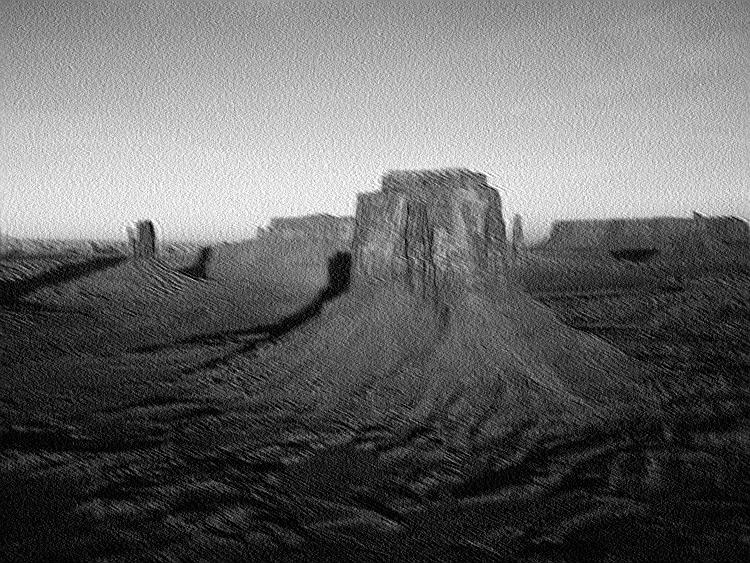
\includegraphics[{width= \textwidth}]{../Images/Results/desert/Gauss/W.png}

\caption{Image deblurred with Wiener (Gaussian noise)}
\label{fig:GaussW}
\end{subfigure}
~
\begin{subfigure}{0.32\textwidth}
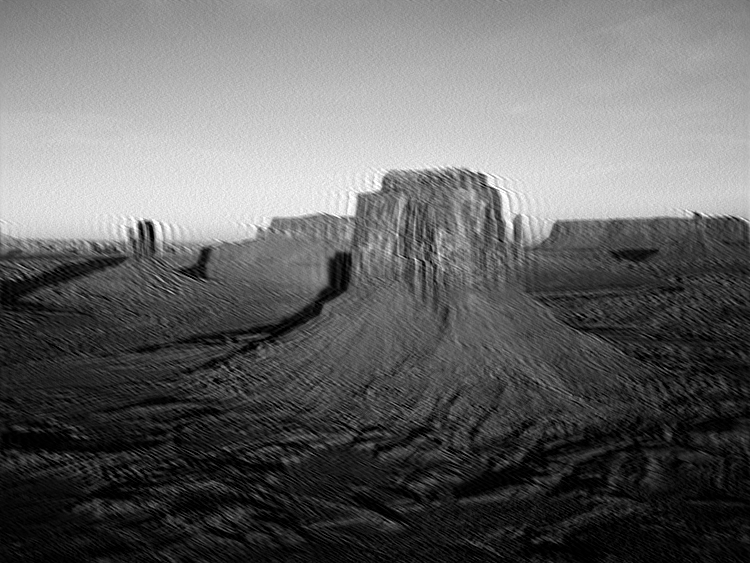
\includegraphics[{width= \textwidth}]{../Images/Results/desert/Speckle/W.png}
\caption{Image deblurred with Wiener (Speckle noise)}
\label{fig:SpeckleW}
\end{subfigure}
~
\begin{subfigure}{0.32\textwidth}
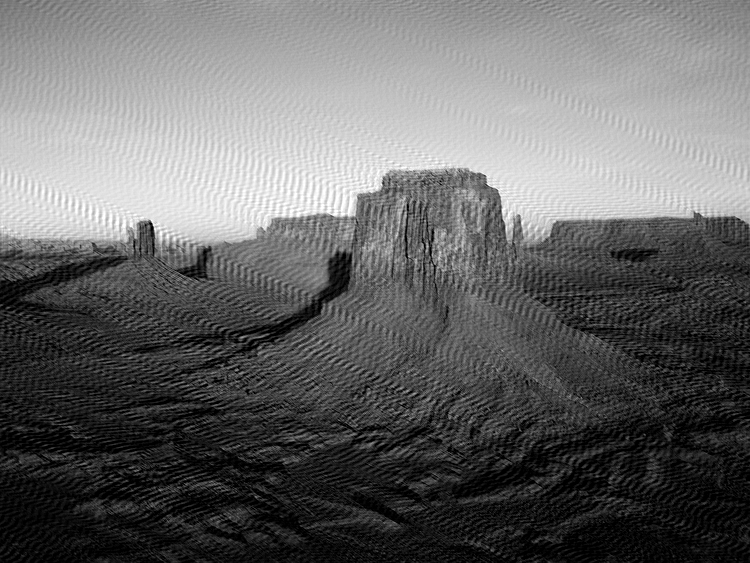
\includegraphics[{width= \textwidth}]{../Images/Results/desert/Normal/R.png}
\caption{Image deblurred with Reguralization (No noise)}
\label{fig:NormalR}
\end{subfigure}
~
\begin{subfigure}{0.32\textwidth}
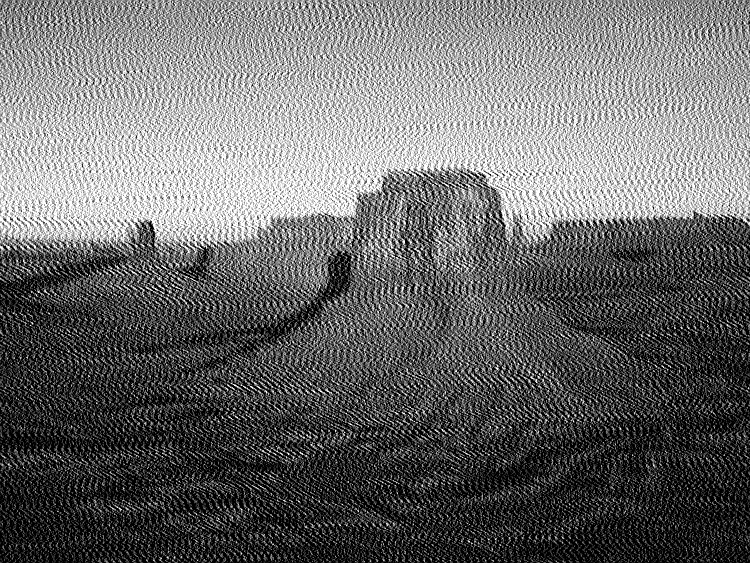
\includegraphics[{width= \textwidth}]{../Images/Results/desert/Gauss/R.png}
\caption{Image deblurred with Reguralization (Gaussian noise)}
\label{fig:GaussR}
\end{subfigure}
~
\begin{subfigure}{0.32\textwidth}
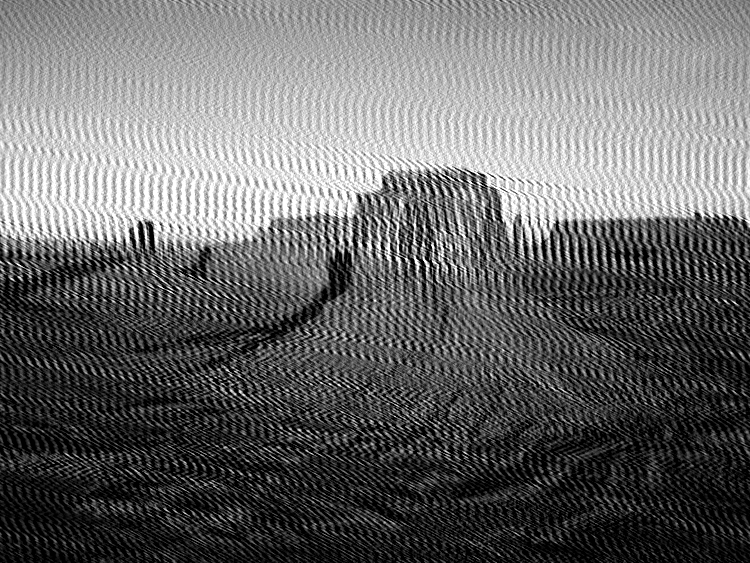
\includegraphics[{width= \textwidth}]{../Images/Results/desert/Speckle/R.png}
\caption{Image deblurred with Reguralization (Speckle noise)}
\label{fig:SpeckleR}
\end{subfigure}
\caption{Left: no noise, center: Gaussian noise, right: Speckle noise}
\label{fig:AllNoises}
\end{figure}


We note that the regularisation algorithm is much more sensitive to both type of noise added in the original image. The other two methods are also affected but the deblurring is not compromised (provided that the initial noise is not too important). This result may be due to wrong coefficients in the equation \eqref{eq:FReg}.
For example the $\alpha$ could not penalize enough the high frequencies.
 
\begin{equation*}
\hat{F}(k,l) = \frac{H(k,l)}{|H(k,l)|^2 + \alpha |L(k,l)|^2} G(k,l)
\label{eq:FReg}
\end{equation*}

\subsection{Length estimation}
\label{subsec:LengthEs}
To estimate the PSF, it is necessary to estimate the length of the psf  as explained in subsection \ref{subsec:Cep}. It's interesting to study the impact of the accuracy of this factor on the output and establish the sensitivity of the three methods used.

The image used here is the famous photo taken in 1972 of Lena, playmate of playboy magazine, and is often used to test algorithms for image processing \cite{wikiLenna}. It has been artificially blurred here with an angle of 20 degrees and a length of 30 pixels, see figure~\ref{fig:LenaBl}. The principle is to fix the estimated length for the deconvolution in order to see the impact on the final result (it should be noted that the angle estimated by this algorithm is 20 degrees which is correct and so the length parameter is the only variable here). For each method, three cases were treated: the estimated length (that is fixed) is 20 pixels, 30 pixels (exact value) and 40 pixels.  The results are shown in figure \ref{fig:LenaGeneral}.

\begin{figure}[h!]
\centering
\begin{subfigure}{0.32\textwidth}
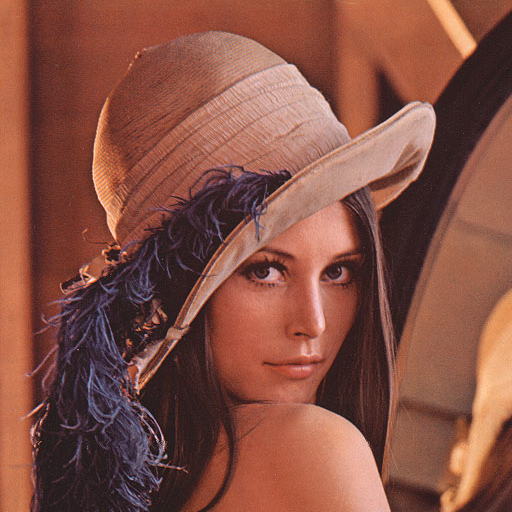
\includegraphics[width= \textwidth]{../Images/Results/Lena/Blur20deg30length/lenaOriginal.png}
\caption{Original image - Lena}
\label{fig:LenaO}
\end{subfigure}
~
\begin{subfigure}{0.32\textwidth}
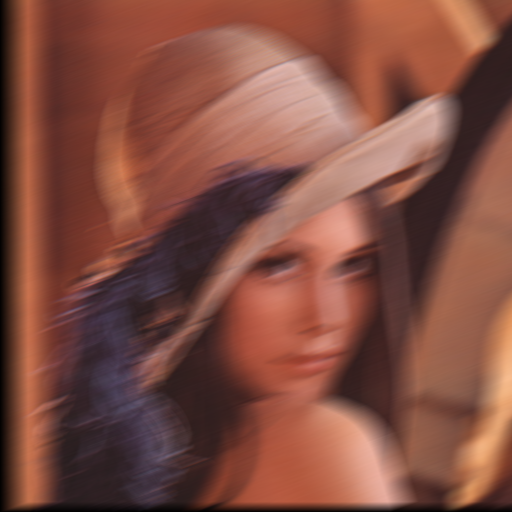
\includegraphics[{width= \textwidth}]{../Images/Results/Lena/Blur20deg30length/ArtificialBlurred.png}
\caption{Artificial blur: $30$ pixels and $0$ degrees}
\label{fig:LenaBlurred}
\end{subfigure}
\caption{Original image (left) and with artificial blur (right)}
\label{fig:LenaBl}
\end{figure}


\begin{figure}[h!]
\centering
\begin{subfigure}{0.32\textwidth}
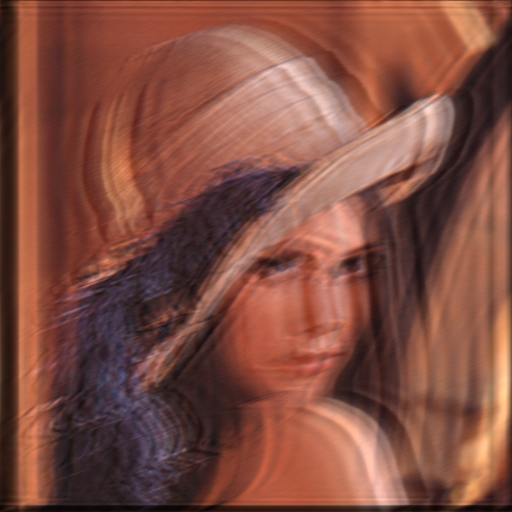
\includegraphics[width= \textwidth]{../Images/Results/Lena/Blur20deg30length/L20.png}
\caption{Lucy if length estimator = $20$ pixels}
\label{fig:L20}
\end{subfigure}
~
\begin{subfigure}{0.32\textwidth}
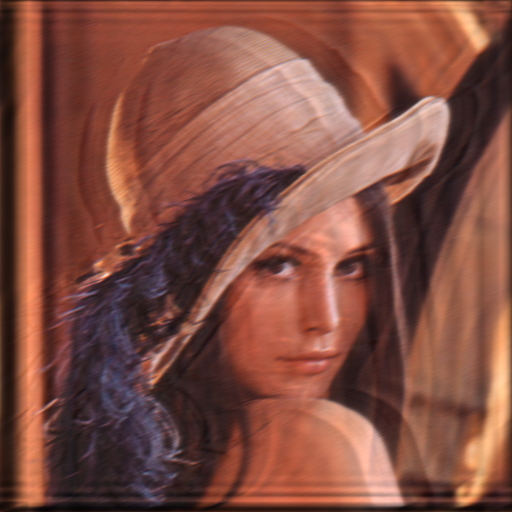
\includegraphics[{width= \textwidth}]{../Images/Results/Lena/Blur20deg30length/L30.png}
\caption{Lucy if length estimator = $30$ pixels (exact value)}
\label{fig:L30}
\end{subfigure}
~
\begin{subfigure}{0.32\textwidth}
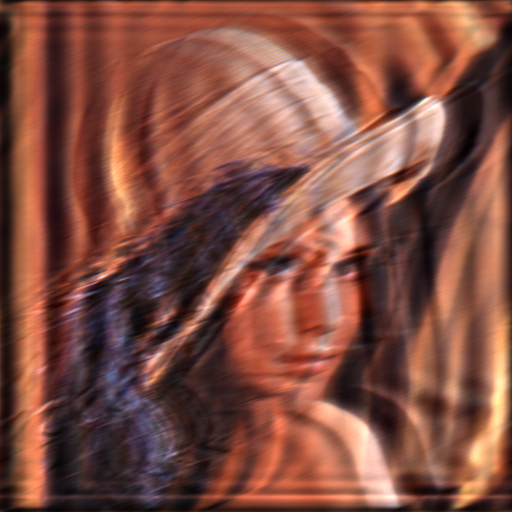
\includegraphics[{width= \textwidth}]{../Images/Results/Lena/Blur20deg30length/L40.png}
\caption{Lucy if length estimator = $40$ pixels}
\label{fig:L40}
\end{subfigure}
~
\begin{subfigure}{0.32\textwidth}
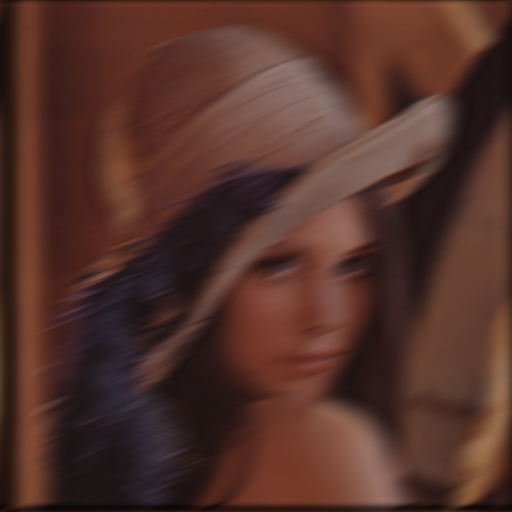
\includegraphics[{width= \textwidth}]{../Images/Results/Lena/Blur20deg30length/W20.png}
\caption{Wiener if length estimator = $20$ pixels}
\label{fig:W20}
\end{subfigure}
~
\begin{subfigure}{0.32\textwidth}
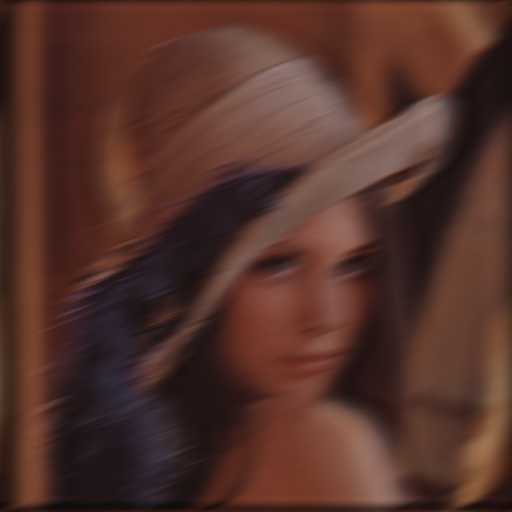
\includegraphics[{width= \textwidth}]{../Images/Results/Lena/Blur20deg30length/W30.png}
\caption{Wiener if length estimator = $30$ pixels (exact value)}
\label{fig:W30}
\end{subfigure}
~
\begin{subfigure}{0.32\textwidth}
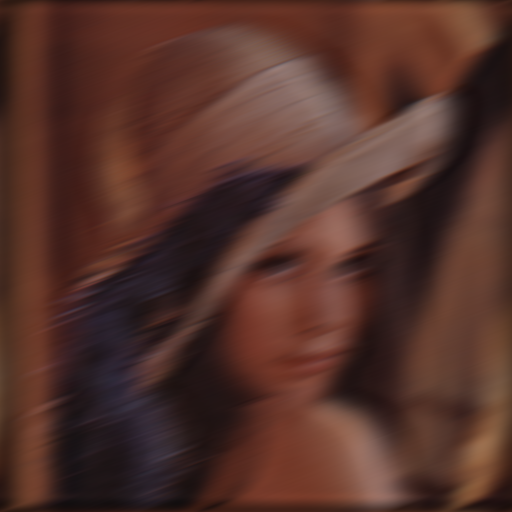
\includegraphics[{width= \textwidth}]{../Images/Results/Lena/Blur20deg30length/W40.png}
\caption{Wiener if length estimator = $40$ pixels.}
\label{fig:W40}
\end{subfigure}
~
\begin{subfigure}{0.32\textwidth}
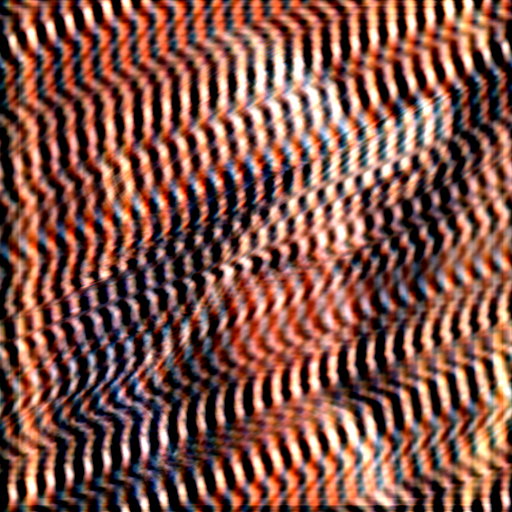
\includegraphics[{width= \textwidth}]{../Images/Results/Lena/Blur20deg30length/R20.png}
\caption{Reguralization if length estimator = $20$ pixels}
\label{fig:R20}
\end{subfigure}
~
\begin{subfigure}{0.32\textwidth}
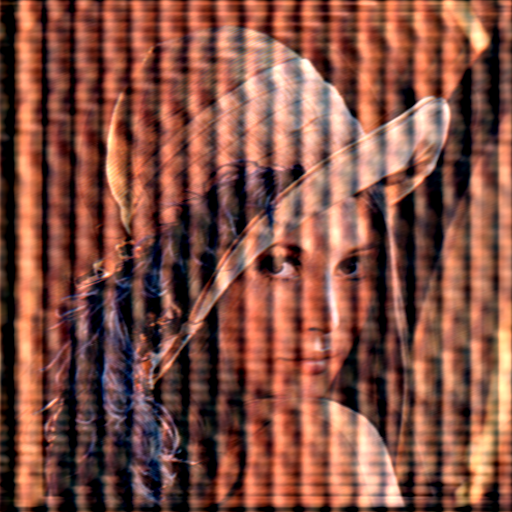
\includegraphics[{width= \textwidth}]{../Images/Results/Lena/Blur20deg30length/R30.png}
\caption{Reguralization if length estimator = $30$ pixels (exact value)}
\label{fig:R30}
\end{subfigure}
~
\begin{subfigure}{0.32\textwidth}
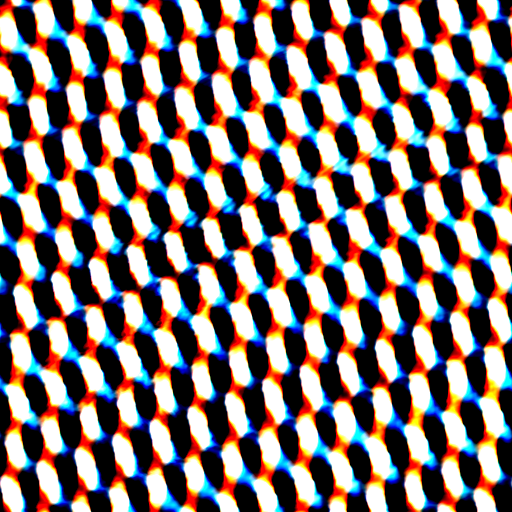
\includegraphics[{width= \textwidth}]{../Images/Results/Lena/Blur20deg30length/R40.png}
\caption{Reguralization if length estimator = $40$ pixels}
\label{fig:R40}
\end{subfigure}
\caption{Influence of the length estimator}
\label{fig:LenaGeneral}
\end{figure}

It directly seems that the regularization method is much more sensitive to the parameter studied than the two others methods. 

Let's focus now on a small variation of the length for regularisation. The following example (figure \ref{fig:PlateReg}) shows that, for an artificially blurred license plate at 0 degree and 40 pixels, the results are already no more relevant with a gap of two pixels. This sensitivity to a small length approximation added to the sensitivity to noise make the regularisation algorithm less efficient than the two others. 

\begin{figure}[h!]
\centering
\begin{subfigure}{0.32\textwidth}

\includegraphics[{width= \textwidth}]{../Images/Results/plaque/Blur0angle40length/originalimage.jpg}
\caption{Original image}
\label{fig:plaqueO}
\end{subfigure}
~
\begin{subfigure}{0.32\textwidth}

\includegraphics[{width= \textwidth}]{../Images/Results/plaque/Blur0angle40length/ArtificialBlur.png}
\caption{Artificial blur: $40$ pixels and $0$ degrees}
\label{fig:plaqueBlur}
\end{subfigure}
\caption{Original image (left) and with artificial blur (right)}
\end{figure}


\begin{figure}[h!]
\center
\begin{subfigure}{0.32\textwidth}
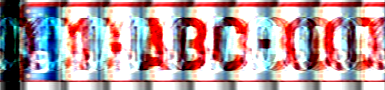
\includegraphics[{width= \textwidth}]{../Images/Results/plaque/Blur0angle40length/RegL38.png}
\caption{Reguralization method with length estimator $= 38$}
\label{fig:RegL38}
\end{subfigure}
~
\begin{subfigure}{0.32\textwidth}
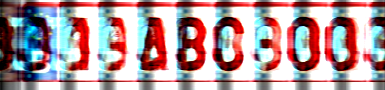
\includegraphics[{width= \textwidth}]{../Images/Results/plaque/Blur0angle40length/RegL39.png}
\caption{Reguralization method with length estimator $= 39$}
\label{fig:RegL39}
\end{subfigure}
~
\begin{subfigure}{0.32\textwidth}

\includegraphics[{width= \textwidth}]{../Images/Results/plaque/Blur0angle40length/RegL40.png}
\caption{Reguralization method with length estimator $= 40$ (exact value)}
\label{fig:RegL40}
\end{subfigure}
~
\begin{subfigure}{0.32\textwidth}
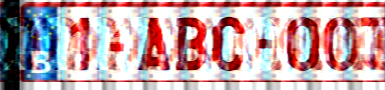
\includegraphics[{width= \textwidth}]{../Images/Results/plaque/Blur0angle40length/RegL41.png}
\caption{Reguralization method with length estimator $= 41$}
\label{fig:RegL41}
\end{subfigure}
~
\begin{subfigure}{0.32\textwidth}
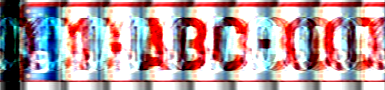
\includegraphics[{width= \textwidth}]{../Images/Results/plaque/Blur0angle40length/RegL42.png}
\caption{Reguralization method with length estimator $= 42$}
\label{fig:RegL42}
\end{subfigure}
\caption{Method of reguralization: influence of the length estimator parameter}
\label{fig:PlateReg}
\end{figure}

\subsection{Angle estimation}
\label{subsec:AngleEs}

After examining the influence of the length, we are interested in the influence of the angle 
estimated with the method of Radon (section~\ref{subsec:Radon}). This parameter is also used in the calculation of the PSF. Moreover, the estimate of the length is possible only after a correct value for the angle. It is therefore all the more important to determine the sensitivity of the methods in this setting because the sensitivity depends on the estimated length.
    
To isolate the parameter, we fix the estimated length as the rigth value for the example used (which is an artificially blurred picture). The test image is a photo artificially blurred whith an angle of 10 degrees and a length of 30 pixels, it represents "la maison caree", in Nîme. The original image and its blurred version is shown in the figure~=\ref{fig:nimeOriginal}. To show its influence, we'll fix the angle parameter to $8$ degrees, $10$ degrees (exact value) and $12$ degrees. The results of deblurring are shown in figure~\ref{fig:NimeGeneral}.

\begin{figure}[h!]
\centering
\begin{subfigure}{0.32\textwidth}
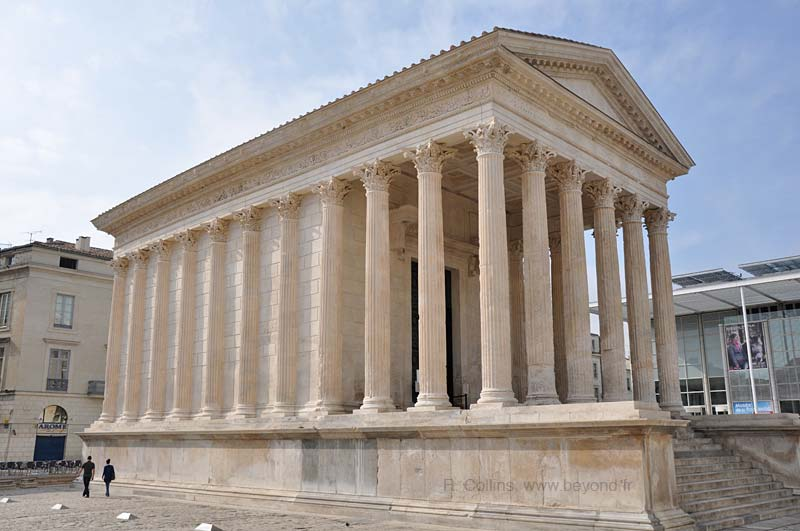
\includegraphics[{width= \textwidth}]{../Images/Results/Nime/Original.jpg}
\caption{Original image}
\label{fig:NimeO}
\end{subfigure}
~
\begin{subfigure}{0.32\textwidth}
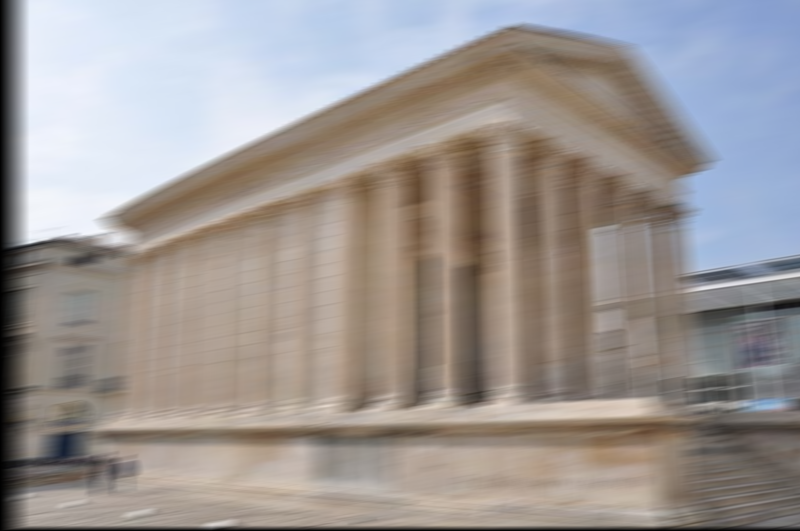
\includegraphics[{width= \textwidth}]{../Images/Results/NimeAngle/Blurlength30angle10.png}
\caption{Artificial blur: $30$ pixels and $10$ degrees}
\label{fig:Blurlength30angle10}
\end{subfigure}
\caption{Original image (left) and with artificial blur (right)}
\label{fig:nimeOriginal}
\end{figure}

\begin{figure}[h!]
\centering
\begin{subfigure}{0.32\textwidth}
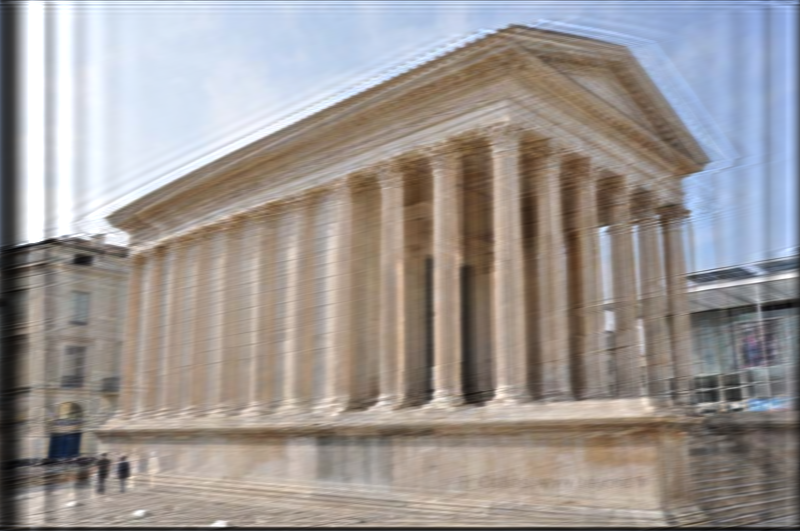
\includegraphics[width= \textwidth]{../Images/Results/NimeAngle/LucyAngle8.png}
\caption{Lucy if angle estimator = $8$ degrees}
\label{fig:L8}
\end{subfigure}
~
\begin{subfigure}{0.32\textwidth}
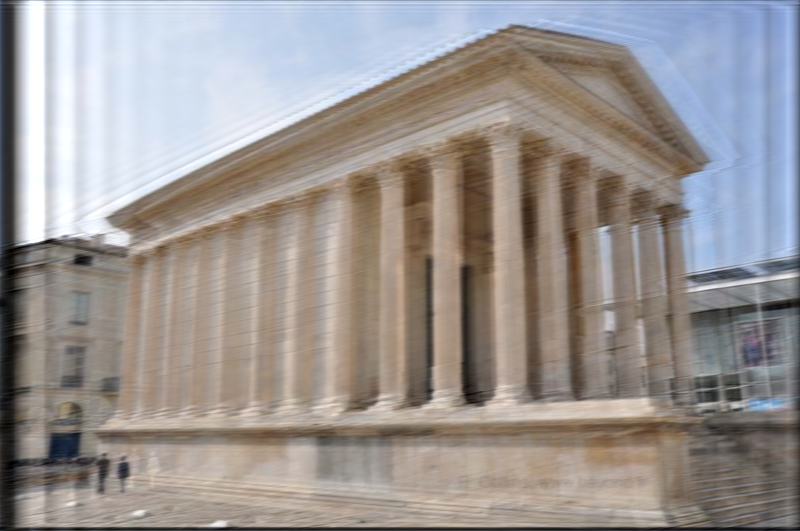
\includegraphics[{width= \textwidth}]{../Images/Results/NimeAngle/WienerAngle8.png}
\caption{Wiener if angle estimator = $8$ degrees}
\label{fig:W8}
\end{subfigure}
~
\begin{subfigure}{0.32\textwidth}
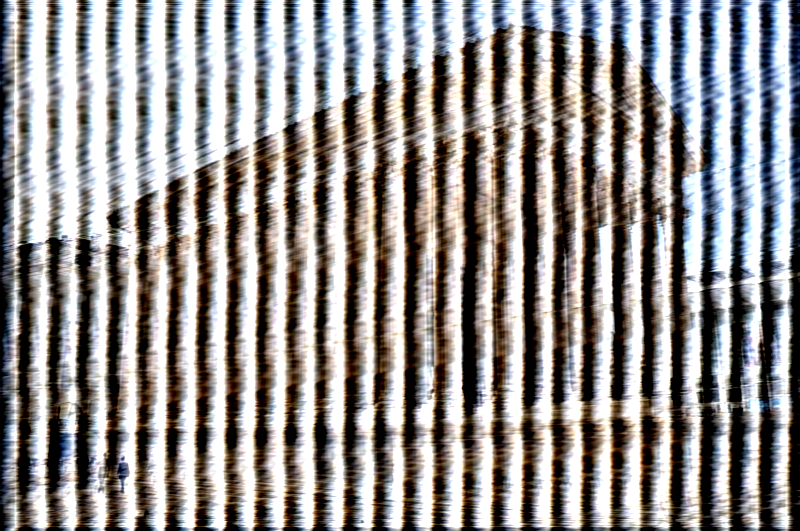
\includegraphics[{width= \textwidth}]{../Images/Results/NimeAngle/RegAngle8.png}
\caption{Reguralization if angle estimator = $8$ degrees}
\label{fig:R8}
\end{subfigure}
~
\begin{subfigure}{0.32\textwidth}
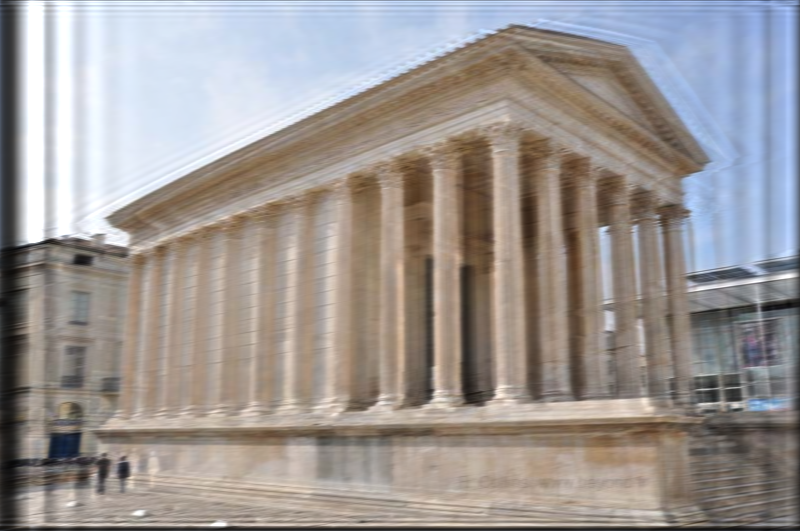
\includegraphics[{width= \textwidth}]{../Images/Results/NimeAngle/LucyAngle10.png}
\caption{Lucy if angle estimator = $10$ degrees}
\label{fig:L10}
\end{subfigure}
~
\begin{subfigure}{0.32\textwidth}
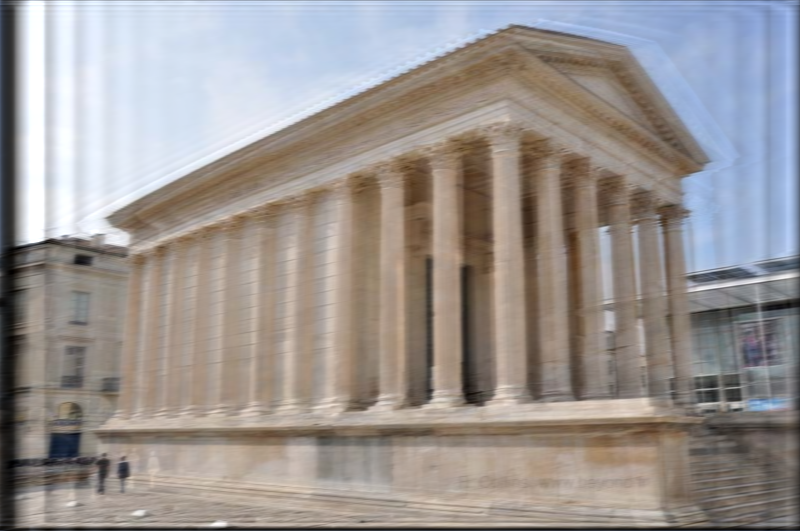
\includegraphics[{width= \textwidth}]{../Images/Results/NimeAngle/WienerAngle10.png}
\caption{Wiener if angle estimator = $10$ degrees}
\label{fig:W10}
\end{subfigure}
~
\begin{subfigure}{0.32\textwidth}
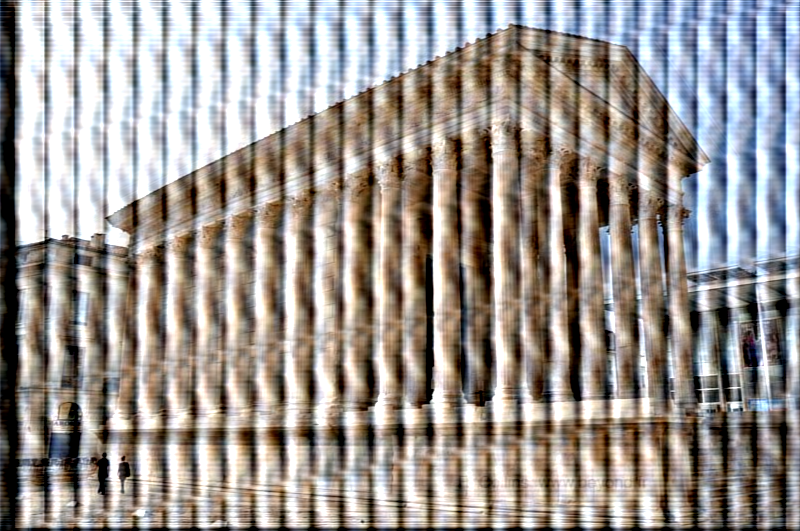
\includegraphics[{width= \textwidth}]{../Images/Results/NimeAngle/RegAngle10.png}
\caption{Reguralization if angle estimator = $10$ degrees}
\label{fig:R10}
\end{subfigure}
~
\begin{subfigure}{0.32\textwidth}
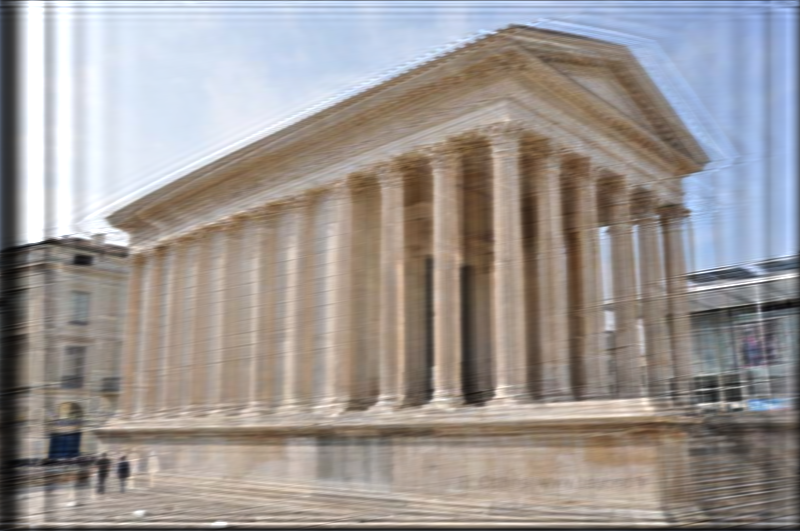
\includegraphics[{width= \textwidth}]{../Images/Results/NimeAngle/LucyAngle12.png}
\caption{Lucy if angle estimator = $12$ degrees}
\label{fig:L12}
\end{subfigure}
~
\begin{subfigure}{0.32\textwidth}
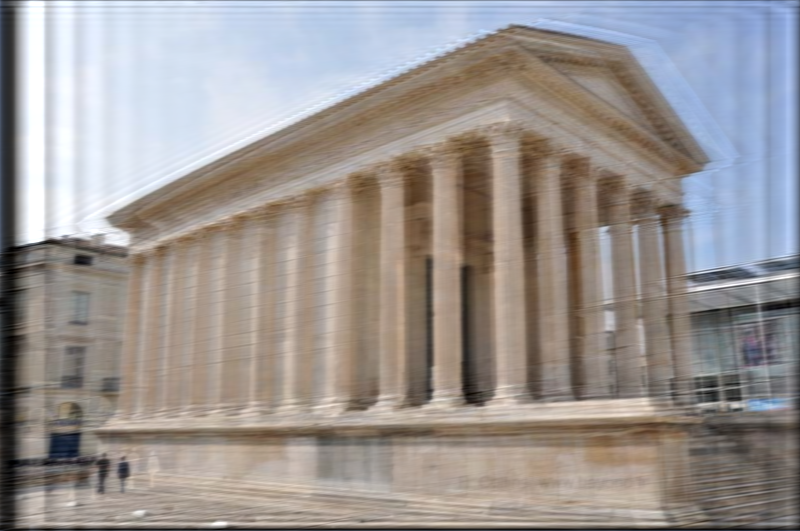
\includegraphics[{width= \textwidth}]{../Images/Results/NimeAngle/WienerAngle12.png}
\caption{Wiener if angle estimator = $12$ degrees}
\label{fig:W12}
\end{subfigure}
~
\begin{subfigure}{0.32\textwidth}
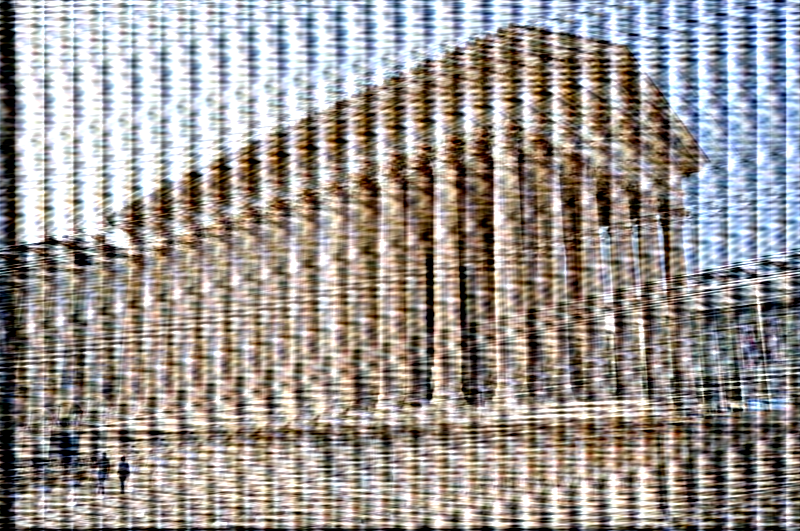
\includegraphics[{width= \textwidth}]{../Images/Results/NimeAngle/RegAngle12.png}
\caption{Reguralization if angle estimator = $12$ degrees}
\label{fig:R12}
\end{subfigure}
\caption{Influence of the length estimator}
\label{fig:NimeGeneral}
\end{figure}

It follows immediately that, in the same way that the estimated length, the regularization method is particularly sensitive to the angle parameter. Indeed, there is much more artefacs when the estimated distance from the exact valeure is important. 
The other two methods, Lucy and Wiener are robust enough once again. Although obviously the deblurring will be better when the estimated value is close to the exact value. 

Conclude by noting that poor estimation of the angle leads to an even worse estimate of the length (which is based on the estimation of the angle). Regularization is even more sensitive to the value of the angle.

\subsection{Influence of the peaks on the length estimation}

As explained in subsection \ref{subsec:Cep}, computing the length of the psf requires searching different peaks. Even if in most of the cases, the estimated length is accurate, we get sometimes some problems. For example if we blur the license plate \ref{fig:plaqueO} with 19 or 21 pixels and k equals 8 (cf. subsection \ref{subsec:Cep} for its meaning), we obtain the exact number, whereas when we blur with 20 pixels, the estimated length is 36 pixels and the deblurred image is less relevant as shown in figure \ref{fig:PlateLen8}. However if we change k to 5, we get 20 pixels estimated and the deblurred image is clearer, figure \ref{fig:PlateLen5}. 

\begin{figure}[h]
\centering
\begin{subfigure}{0.32\textwidth}

\includegraphics[{width= \textwidth}]{../Images/Results/plaque/20/Lucyblur19estimated19k3.png}
\caption{Deblurring (Lucy) for artificial blur of $19$ pixels with $k=8$ (length estimation = $19$ pixels)}
\label{fig:LB19E19K3}
\end{subfigure}
~
\begin{subfigure}{0.32\textwidth}

\includegraphics[{width= \textwidth}]{../Images/Results/plaque/20/Lucyblur20estimation36k3.png}
\caption{Deblurring (Lucy) for artificial blur of $20$ pixels with $k=8$ (length estimation = $36$ pixels)}
\label{fig:LB20E36K3}
\end{subfigure}
~
\begin{subfigure}{0.32\textwidth}

\includegraphics[{width= \textwidth}]{../Images/Results/plaque/20/Lucyblur21estimated21k3.png}
\caption{Deblurring (Lucy) for artificial blur of $21$ pixels with $k=8$ (length estimation = $21$ pixels)}
\label{fig:LB21E21K3}
\end{subfigure}
\caption{Compression: Deblurring (Lucy) for different length of artificial blur for $k = 3$}
\label{fig:PlateLen8}
\end{figure}

\begin{figure}[h]
\centering

\includegraphics[{width= 0.4\textwidth}]{../Images/Results/plaque/20/LucyBlur20estimation20k2.png}
\caption{Deblurring (Lucy) for artificial blur of $20$ pixels with $k=5$ (length estimated = $20$ pixels)}
\label{fig:PlateLen5}
\end{figure}


If we check the graphs of the peaks of the modified cepstrum, figure \ref{fig:PlatePeaks}, it is clear that the graphs \ref{fig:peaksLucy19} and \ref{fig:peaksLucy21} are sharper than the graph \ref{fig:peaksLucy20} which explain that to find a peak with more than 8 pixels independent of the principal peak is problematic. This problem is one of the inefficiencies we could try to manage in a future version of our algorithm. Indeed, for the moment, we just let the possibility for the user to adjust manually this parameter. 

\begin{figure}[h]
\centering
\begin{subfigure}{0.32\textwidth}
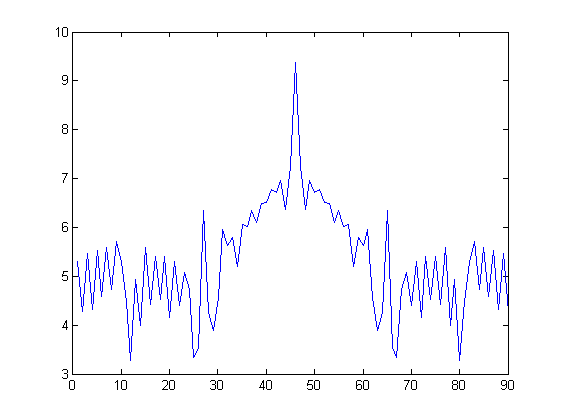
\includegraphics[{width= \textwidth}]{../Images/Results/plaque/20/PicsLucy19.png}
\caption{peaks for artificial blur of $19$ pixels}
\label{fig:peaksLucy19}
\end{subfigure}
~
\begin{subfigure}{0.32\textwidth}
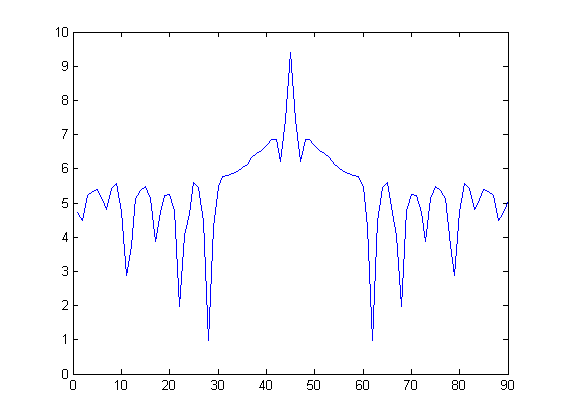
\includegraphics[{width= \textwidth}]{../Images/Results/plaque/20/PicsLucy20.png}
\caption{peaks for artificial blur of $20$ pixels)}
\label{fig:peaksLucy20}
\end{subfigure}
~
\begin{subfigure}{0.32\textwidth}
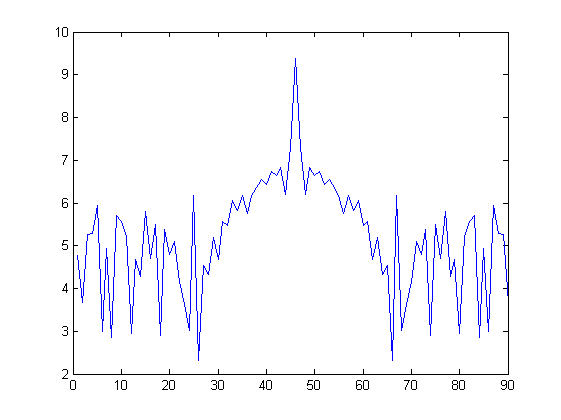
\includegraphics[{width= \textwidth}]{../Images/Results/plaque/20/PicsLucy21.png}
\caption{Peaks for artificial blur of $21$ pixels}
\label{fig:peaksLucy21}
\end{subfigure}
\caption{peaksLucy}
\label{fig:PlatePeaks}
\end{figure}

\subsection{Compression and computation time}

Our bonus item relates to the computation time of deblurring. It's important to analyse whether the time saved is significant and if it's not compromising quality of deblurred images. So we will compare the computing time  for the three algorithms with and without the psf estimation on a smaller part of the picture and resizing . The testing picture is the photo of Lena, artificially blurred with an angle of 50 degrees and with a length of 80 pixels. We estimate the psf on a square of $256 \times 256$ pixels and we resize the picture from $1400 \times 1400 \times 3$ to $750 \times 750 \times 3$ pixels.

The following table shows the different computation time:

\begin{center}
\begin{tabular}{|l|c|c|r|}
  \hline
  & Lucy &  Wiener & regularization \\
  \hline
  Time with compression [s] & 5.78 & 0.69 & 2.11 \\
  \hline
  Time without compression [s]  & 18.99 & 2.77 & 6.12 \\
  \hline
\end{tabular}
\end{center}


\begin{figure}[h]
\centering
\begin{subfigure}{0.32\textwidth}
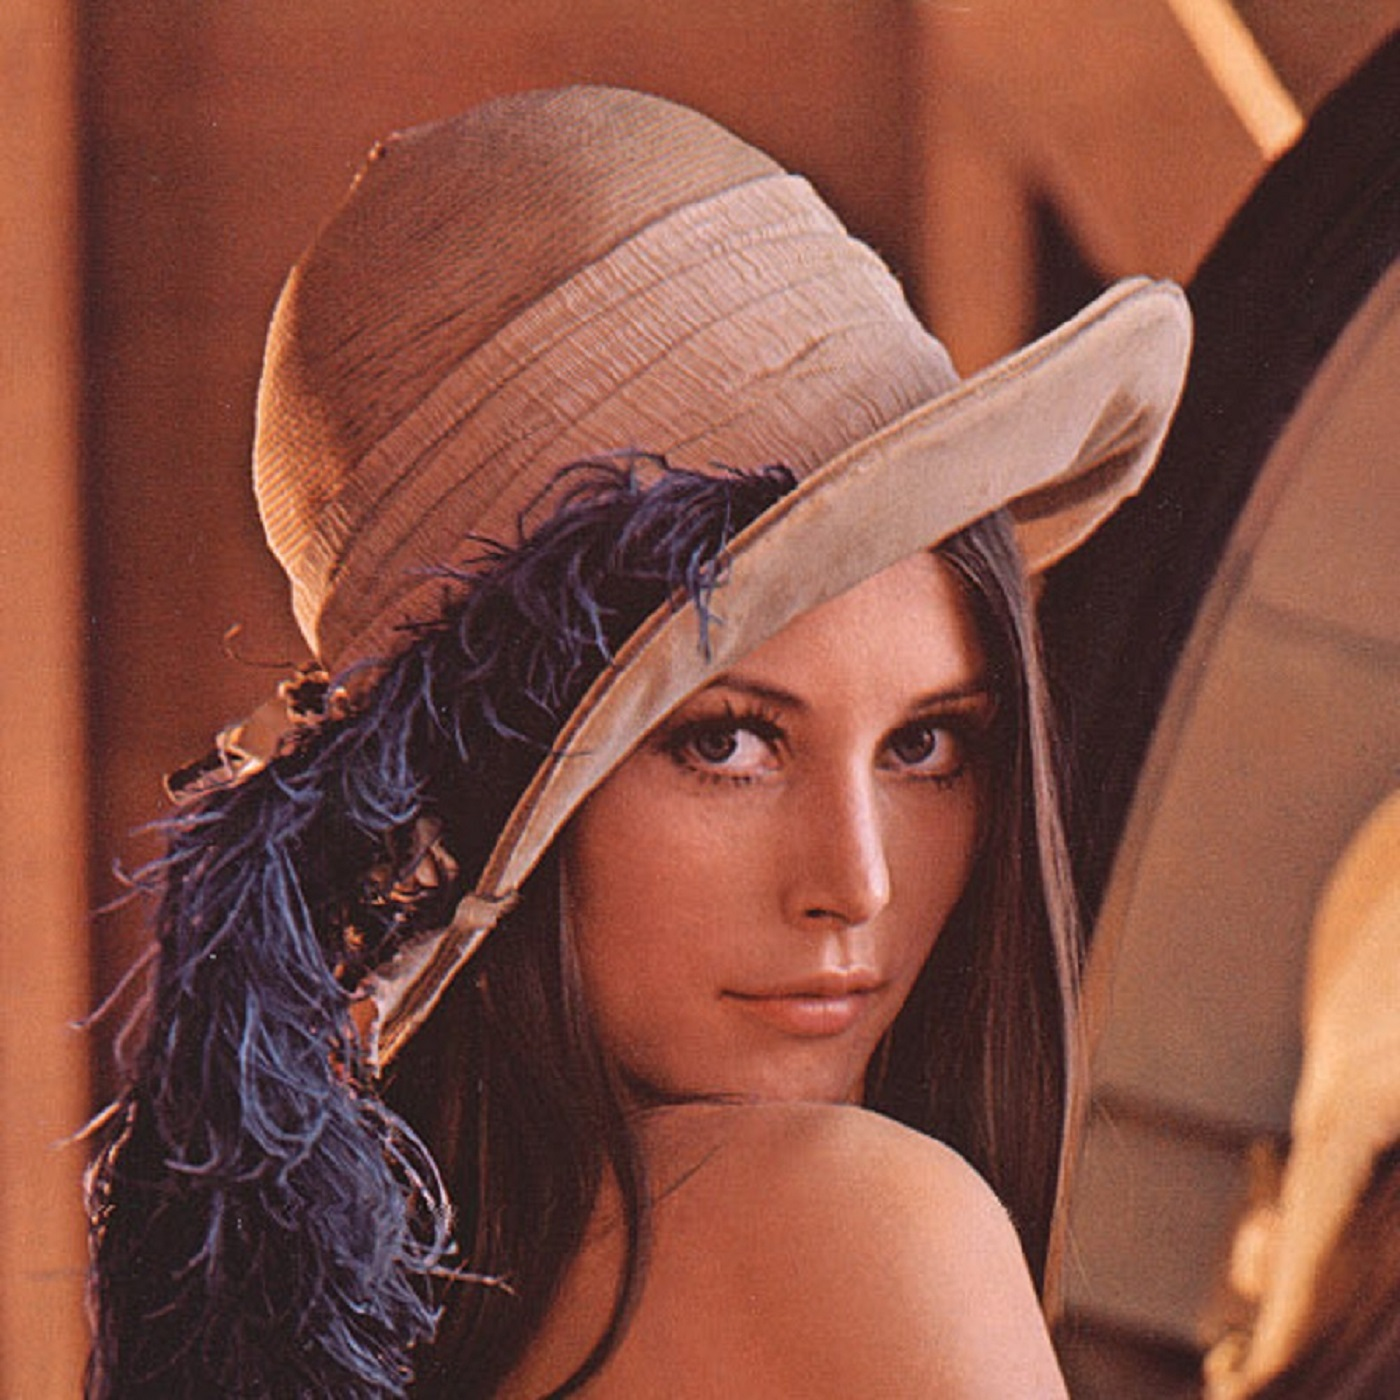
\includegraphics[{width= \textwidth}]{../Images/Results/Lena/Lena2/lena.jpg}
\caption{Original image - Lena}
\label{fig:LenaO}
\end{subfigure}
~
\begin{subfigure}{0.32\textwidth}
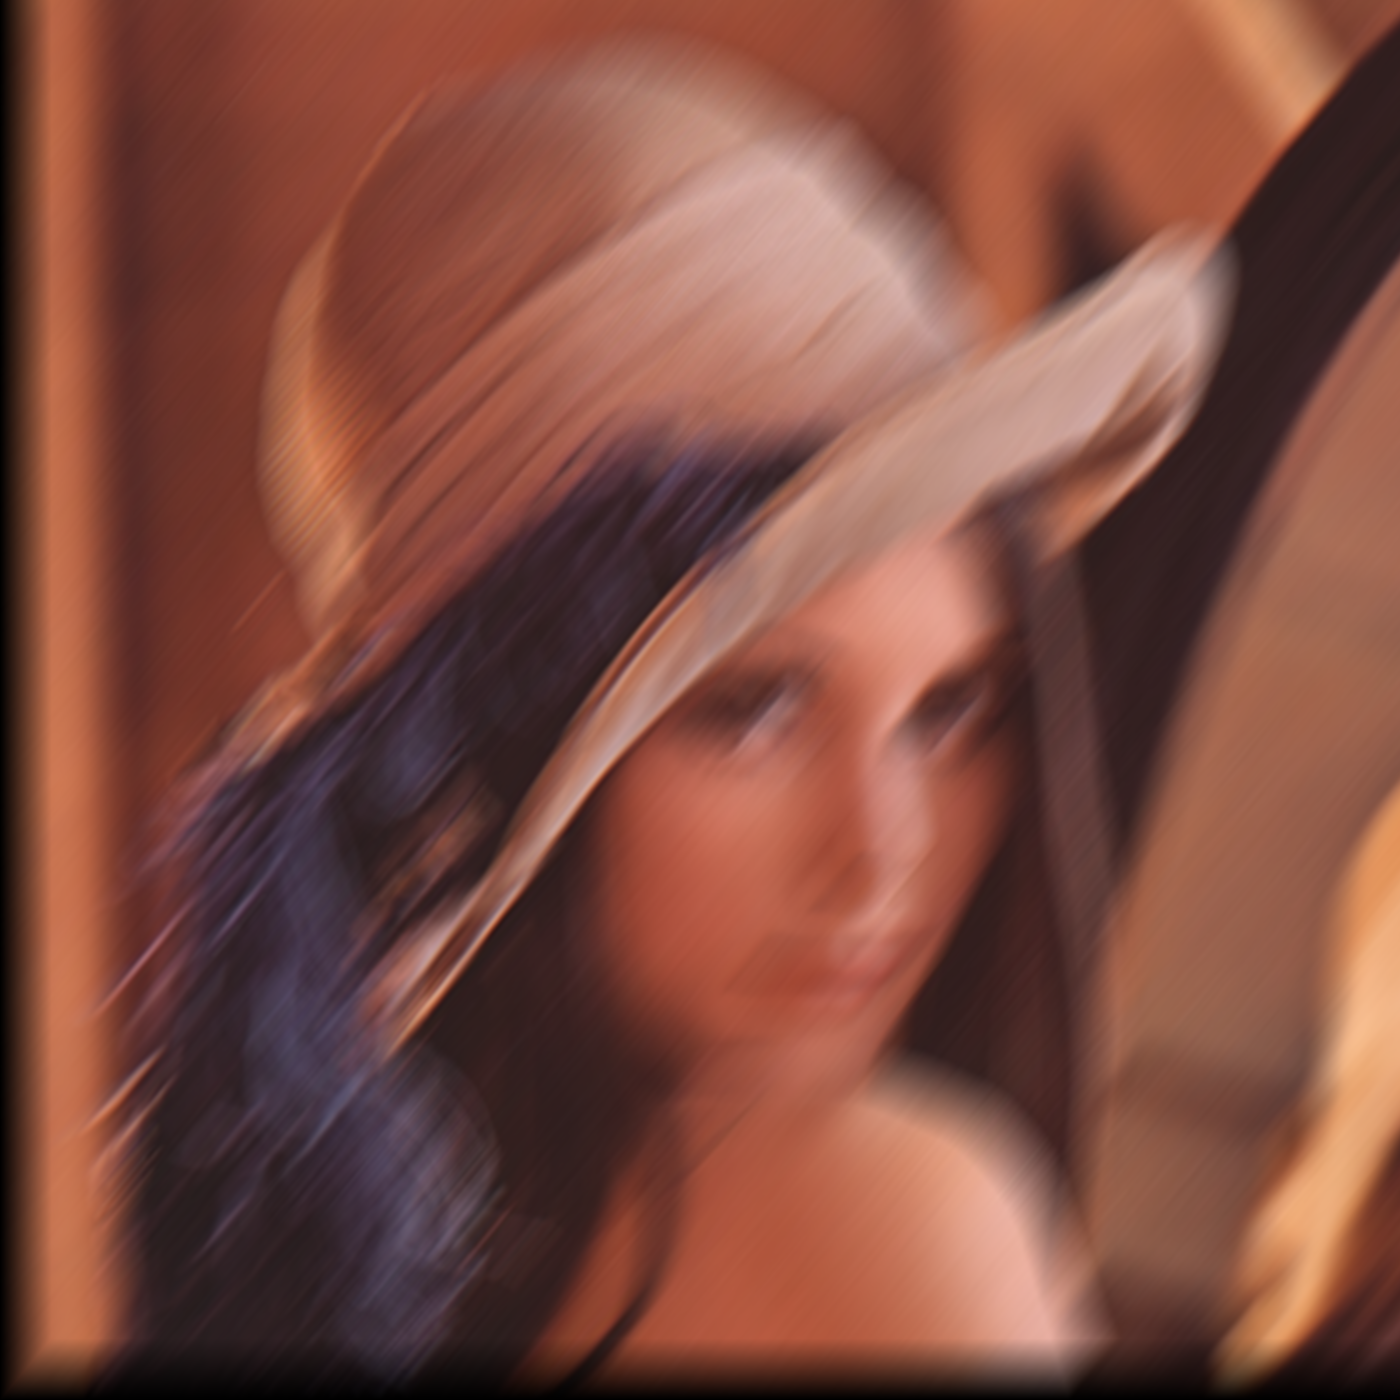
\includegraphics[{width= \textwidth}]{../Images/Results/Lena/Lena2/Blur80a50.png}
\caption{Artificial blur: $80$ pixels and $50$ degrees}
\label{fig:Blur80a50}
\end{subfigure}
\caption{Original image (left) and with artificial blur (right)}
\end{figure}

\begin{figure}[h]
\centering
\begin{subfigure}{0.32\textwidth}
\includegraphics[{width= \textwidth}]{../Images/Results/Lena/Lena2/Lucy.png}
\caption{Picture deblurred with Lucy (16 iterations)}
\label{fig:Lulu}
\end{subfigure}
~
\begin{subfigure}{0.32\textwidth}
\includegraphics[{width= \textwidth}]{../Images/Results/Lena/Lena2/Wiener.png}
\caption{Picture deblurred with Wiener}
\label{fig:Wiwi}
\end{subfigure}
~
\begin{subfigure}{0.32\textwidth}
\includegraphics[{width= \textwidth}]{../Images/Results/Lena/Lena2/Reg.png}
\caption{Picture deblurred with Reguralization}
\label{fig:Rere}
\end{subfigure}
~
\begin{subfigure}{0.32\textwidth}
\includegraphics[{width= \textwidth}]{../Images/Results/Lena/Lena2/Lucy-Comp.png}
\caption{Picture deblurred with Lucy (compressing process)}
\label{fig:Lucycomp}
\end{subfigure}
~
\begin{subfigure}{0.32\textwidth}
\includegraphics[{width= \textwidth}]{../Images/Results/Lena/Lena2/Wiener-Comp.png}
\caption{Picture deblurred with Wiener (compressing process)}
\label{fig:Wienercomp}
\end{subfigure}
~
\begin{subfigure}{0.32\textwidth}
\includegraphics[{width= \textwidth}]{../Images/Results/Lena/Lena2/Reg-Comp.png}
\caption{Picture deblurred with Reguralization (compressing process)}
\label{fig:Regcom}
\end{subfigure}
\caption{Compression: comparison of results}
\end{figure}


We see that in this case the compression significantly reduces the computation time with only small visible differences between the deblurred image with and without \texttt{compression.m} (more artifacts for reguralisation with the  process). 
However, in some cases the angle and length estimations can be less accurate (around $\pm$ 1 degree and $\pm$ 3 pixels). As shown in subsections \ref{subsec:LengthEs} and \ref{subsec:AngleEs} it's mainly problematic for the regularisation algorithm.

\subsection{Complexity of our different results}

As the time spent for the psf estimation and the resizing is the same for all the algorithms (around 0.8 seconds), we can conclude that the Lucy-Richardson algorithm is the slowest, around $6 $ seconds for a $750 \times 750 \times 3$ color picture and 16 iterations. The wiener algorithm is the fastest with less than $0.5$ second in average. Finally the regularisation takes about $1.5$ seconds to compute. For a gray scale picture it means only $750 \times 750$, we get $1.4$ seconds for Lucy and 16 iterations, $0.04$ for Wiener and $0.3$ for the regularisation. 

Let's estimate the complexity of the deconvolution algorithms. To do so, we use the same picture. We first deblur the picture using \texttt{deconvlucy} for a certain size($125 \times 125$ here), then for $250 \times 250$, until $2500 \times 2500$ (the original picture  size was $5184 \times 3456$). Afterwards we compute  \texttt{deconvwnr} and \texttt{deconvreg} in the same way. The figure \ref{fig:Complexity} plots the ratio ``time needed to compute the picture/ time needed to compute the smallest picture'' on the y axis and on the x axis the ratio ``number of pixels of the picture / number of pixels of the smallest picture''. 


\begin{figure}[h!]
\centering
\includegraphics[scale=0.7]{../Images/Complexity.png}
\caption{Complexity of our different algorithms. The blue line is for \texttt{deconvLucy}, the red one for \texttt{deconvwnr} and the green one for \texttt{deconvreg}. the ratio ``time needed to compute the picture/ time needed to compute the smallest picture'' is the y axis and the x axis is the ratio ``number of pixels of the picture / number of pixels of the smallest picture''.}
\label{fig:Complexity}
\end{figure}

\todo{tirer des conclusions}

Let's now have a look at the complexity of our \texttt{robust\_ angle\_ estimator} and \texttt{length \_ estimator} methods. Proceeding in the same way as for the deconvolution algorithms, we 


\begin{figure}[h!]
\centering
\includegraphics[scale=0.7]{../Images/ComplexityRadon.png}
\caption{Complexity of our }
\label{fig:ComplexityRadon}
\end{figure}

\todo{tirer des conclusions}

%\subsection{Colors influence}
%
%First of all, there is an influence on the run time. Indeed, as already seen ([MATH section]), color images are stored in 3-dimensions matrix $M$ x $N$ x $3$. So they take longer to be processed that the same gray-scaled image, stored in a matrix $M$ x $N$.
%Below are the results obtained with the algorithm Lucy-Richardson (with compression) for the photo of Lena and the gray-scaled one corresponding, both artificially blurred with an angle of 50 degrees and a length of 80 pixels:
%
%\begin{figure}[h]
%\centering
%\begin{subfigure}{0.4\textwidth}
%\includegraphics[{width= \textwidth}]{../Images/Results/Lena/Lena2/Blur80a50.png}
%
%\caption{Artificial blur - RGB image}
%\label{fig:B80A50}
%\end{subfigure}
%~
%\begin{subfigure}{0.4\textwidth}
%\includegraphics[{width= \textwidth}]{../Images/Results/Lena/Lena2/Lucy.png}
%
%\caption{Lucy with the RGB image}
%\label{fig:LucyC}
%\end{subfigure}
%~
%\begin{subfigure}{0.4\textwidth}
%\includegraphics[{width= \textwidth}]{../Images/Results/Lena/Lena2/Blur80a50NB.png}
%
%\caption{Artificial blur - gray-scaled image}
%\label{fig:B80A50NB}
%\end{subfigure}
%~
%\begin{subfigure}{0.4\textwidth}
%\includegraphics[{width= \textwidth}]{../Images/Results/Lena/Lena2/LucyNB.png}
%
%\caption{Lucy with the gray-scaled image}
%\label{fig:LNBn}
%\end{subfigure}
%\caption{Computation time for the RGB image: $6,98$[s]; for gray-scaled one: $2,41$[s]}
%\end{figure}
%
%%TODO voir pourquoi Wiener beug parfois selon les couleurs



\subsection{reals images}

\begin{figure}[h]
\centering
\begin{subfigure}{0.4\textwidth}
\includegraphics[{width= \textwidth}]{../Images/Results/reel/foot/Original.jpg}

\caption{Original image (natural blur)}
\label{fig:footOriginal}
\end{subfigure}
~
\begin{subfigure}{0.4\textwidth}
\includegraphics[{width= \textwidth}]{../Images/Results/reel/foot/L.png}

\caption{Lucy}
\label{fig:footLucy}
\end{subfigure}
~
\begin{subfigure}{0.4\textwidth}
\includegraphics[{width= \textwidth}]{../Images/Results/reel/foot/W.png}

\caption{Wiener}
\label{fig:footWiener}
\end{subfigure}
~
\begin{subfigure}{0.4\textwidth}
\includegraphics[{width= \textwidth}]{../Images/Results/reel/foot/Reg.png}

\caption{Regularization}
\label{fig:footReg}
\end{subfigure}
\caption{Deblurring of a poster (natural blur)}
\end{figure}

\begin{figure}[h]
\centering
\begin{subfigure}{0.4\textwidth}
\includegraphics[{width= \textwidth}]{../Images/Results/reel/Mur/Original.jpg}

\caption{Original image (natural blur)}
\label{fig:murOriginal}
\end{subfigure}
~
\begin{subfigure}{0.4\textwidth}
\includegraphics[{width= \textwidth}]{../Images/Results/reel/Mur/L.png}

\caption{Lucy}
\label{fig:murLucy}
\end{subfigure}
~
\begin{subfigure}{0.4\textwidth}
\includegraphics[{width= \textwidth}]{../Images/Results/reel/Mur/W.png}

\caption{Wiener}
\label{fig:murWiener}
\end{subfigure}
~
\begin{subfigure}{0.4\textwidth}
\includegraphics[{width= \textwidth}]{../Images/Results/reel/Mur/R.png}

\caption{Reguralization}
\label{fig:murReg}
\end{subfigure}
\caption{Deblurring of a wall (real noise)}
\end{figure}

 
The results are pretty conclusive so far as the original blurred follows a minimum the assumptions which is not always given. Generally, Reguralisation is not valid for real images, this is explained by the fact that this method is very sensitive to the length parameter estimation and noise. However, in an image with a real blur, it's more difficult to properly estimate the length (blur not linear, "speed" of blurring non-constant) and the noise is very present (including photos taken above by a amateur camera). Lucy and Wiener are stronger, making it more interesting algorithm. However, Lucy is better than Wiener, but in return the execution time is more important.

\subsection{conclusion}

The three methods each have their advantages and disadvantages. Reguralization method is fast but too sensitive to noise and estimation of length, it's so not very robust but still interesting from a theoretical perspective. By contrast, The other two methods are robust. Wiener has the advantage of being faster than Lucy but the results are generally worse than those of Lucy.

\begin{figure}[h]
\centering
\begin{subfigure}{0.32\textwidth}
\includegraphics[{width= \textwidth}]{../Images/Results/fleur/Original.jpg}

\caption{Original image}
\label{fig:fleurO}
\end{subfigure}
~
\begin{subfigure}{0.32\textwidth}
\includegraphics[{width= \textwidth}]{../Images/Results/fleur/B40.png}

\caption{Artificial blur: $40$ pixels and $0$ degrees}
\label{fig:fleurBlur}
\end{subfigure}
\caption{Original image (left) and with artificial blur (right)}
\end{figure}

\begin{figure}[h]
\centering
\begin{subfigure}{0.32\textwidth}
\includegraphics[{width= \textwidth}]{../Images/Results/fleur/L.png}

\caption{Lucy}
\label{fig:fleurL}
\end{subfigure}
~
\begin{subfigure}{0.32\textwidth}
\includegraphics[{width= \textwidth}]{../Images/Results/fleur/W.png}

\caption{Wiener}
\label{fig:fleurW}
\end{subfigure}
~
\begin{subfigure}{0.32\textwidth}
\includegraphics[{width= \textwidth}]{../Images/Results/fleur/R.png}

\caption{Reguralization}
\label{fig:fleurR}
\end{subfigure}
\caption{Deblurring of flowers}
\end{figure}

\begin{figure}[h]
\centering
\begin{subfigure}{0.32\textwidth}
\includegraphics[{width= \textwidth}]{../Images/Results/Nime/Original.jpg}

\caption{Original image}
\label{fig:NimeO}
\end{subfigure}
~
\begin{subfigure}{0.32\textwidth}
\includegraphics[{width= \textwidth}]{../Images/Results/Nime/B35.png}

\caption{Artificial blur: $35$ pixels and $0$ degrees}
\label{fig:NimeBlur}
\end{subfigure}
\caption{Original image (left) and with artificial blur (right)}
\end{figure}

\begin{figure}[h]
\centering
\begin{subfigure}{0.32\textwidth}
\includegraphics[{width= \textwidth}]{../Images/Results/Nime/L.png}

\caption{Lucy}
\label{fig:NimeL}
\end{subfigure}
~
\begin{subfigure}{0.32\textwidth}
\includegraphics[{width= \textwidth}]{../Images/Results/Nime/W.png}

\caption{Wiener}
\label{fig:NimeW}
\end{subfigure}
~
\begin{subfigure}{0.32\textwidth}
\includegraphics[{width= \textwidth}]{../Images/Results/Nime/R.png}
\caption{Reguralization}
\label{fig:NimeR}
\end{subfigure}
\caption{Deblurring}
\end{figure}
